\documentclass{beamer}
\usepackage{amsfonts,amsmath,oldgerm}
\usepackage{xspace}
\usepackage{bbm}
\usepackage{tabularx}
\usepackage{booktabs}
\usepackage{adjustbox}
\usetheme{sintef}
\usepackage{tikz}

\usepackage{xeCJK}
\usepackage{multirow}
% table
\usepackage{booktabs}
\usepackage{threeparttable}
% \input{bring-your-own/arXiv-2311.07850v1/math_commands.tex}
% \usepackage{tabularx}

\newcommand{\testcolor}[1]{\colorbox{#1}{\textcolor{#1}{test}}~\texttt{#1}}

% newcommand for red text
\newcommand{\red}[1]{\textcolor{red}{#1}}


\usefonttheme[onlymath]{serif}

\titlebackground*{assets/background}

\newcommand{\hrefcol}[2]{\textcolor{cyan}{\href{#1}{#2}}}
\newcommand*{\rom}[1]{\expandafter\@slowromancap\romannumeral #1@}


\title{Evaluation of Reasoning Ability of Retrieval-based Language Models}
% \course{Master's Degree in Computer Science}
\author{Yantao Liu}
% \IDnumber{1234567}
\date{\today}


\begin{document}
\maketitle

\section{Introduction}
\begin{frame}
\frametitle{What is Retrieval-based Language Models?}
    % color blue
    Retrieval-based LMs = Retrieval + LMs
    \begin{itemize}
        \item It is a \textbf{Language Model} \\
        \begin{center}
            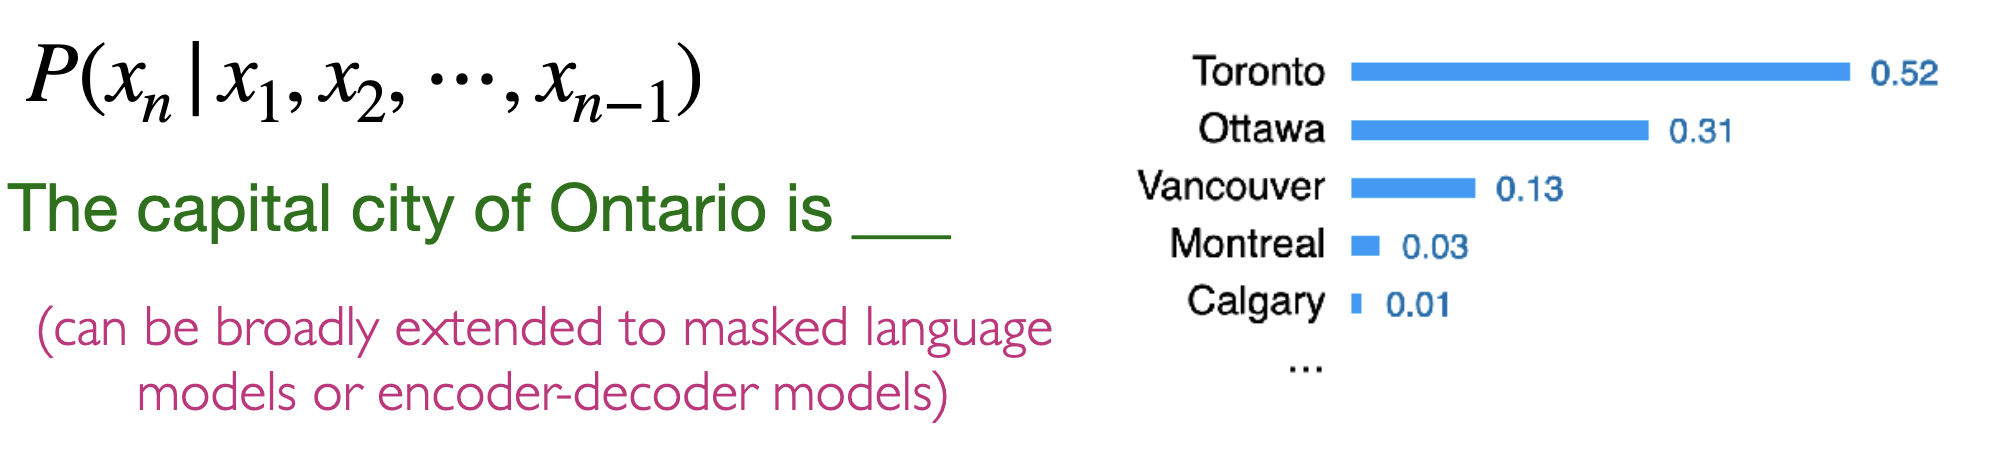
\includegraphics[width=0.6\textwidth]{figure/lm.png}
        \end{center}
        \item It retrieves from an \textbf{external knowledge source} at inference time
        \begin{center}
            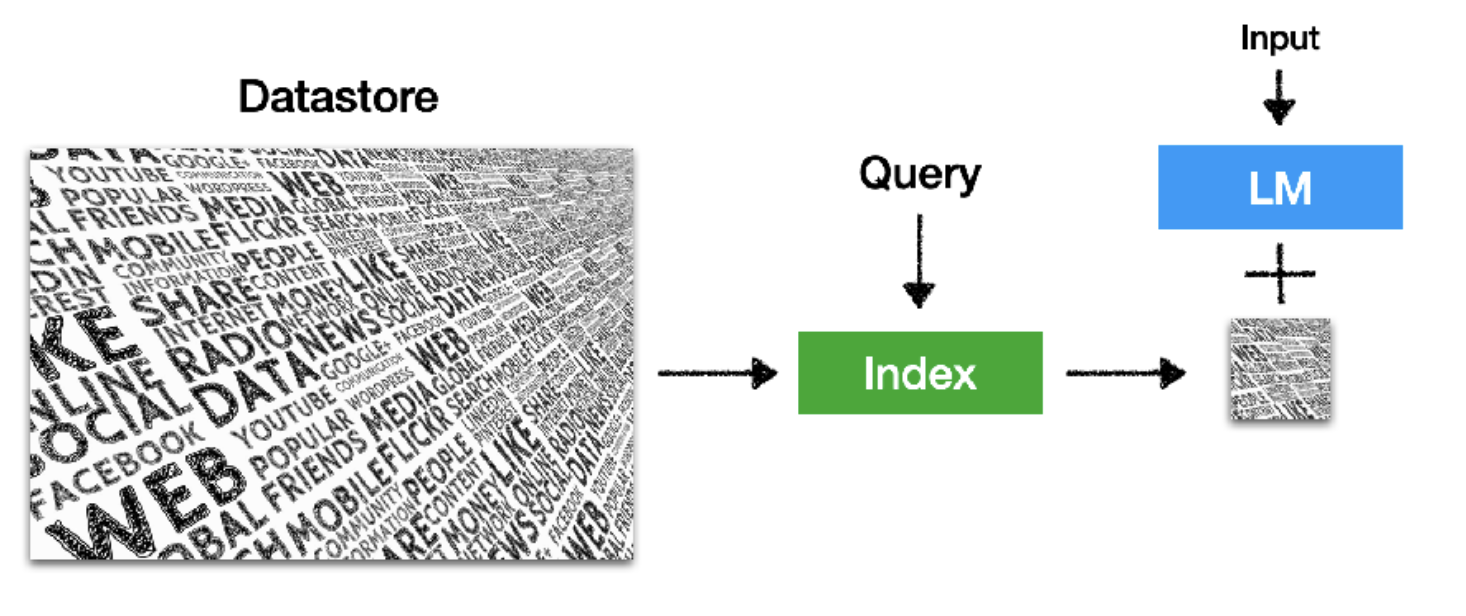
\includegraphics[width=0.6\textwidth]{figure/retrieval.png}
        \end{center}
    \end{itemize}
\end{frame}

\begin{frame}
    \frametitle{Why do we care about the reasoning ability of Retrieval-based LMs?}
    \begin{itemize}
        \item It is a \textbf{Language Model} \\
         --> It already has internal knowledge
        \item It retrieves from an \textbf{external knowledge source} at inference time \\
         --> External knowledge will also be integrated into the model
        \item This leads to the following questions:
    \end{itemize}
    \begin{block}{Interactions between internal and external knowledge}
        \textbf{RQ1:} How well can LMs integrate external knowledge with internal knowledge? \textit{\red{ACL 2023}} \\
        \textbf{RQ2:} How well can LMs reason about conflicting external knowledge? \textit{\red{COLING 2024}} \\
        \textbf{RQ3:} How well can LMs reason about new real-world external knowledge? \textit{\red{ICLR 2024}}
    \end{block}
\end{frame}


\section{KoRC: Knowledge Oriented Reading Comprehension (ACL 2023)}

\begin{frame}
\frametitle{Background}
\begin{itemize}
    \item Existing QA datasets focus on either:
    \begin{itemize}
        \item Extracting knowledge from passages (e.g., SQuAD, HotpotQA).
        \item Evaluating internal knowledge of LLMs (e.g., TriviaQA, Natural Questions).
    \end{itemize}
\end{itemize}

\end{frame}

\begin{frame}
\frametitle{Motivation}
\begin{columns}
    \column{0.5\textwidth}
    % Existing QA datasets either focus on extracting knowledge from the passage (SQuAD, HotpotQA) or examining the internal knowledge of LLMs (TriviaQA, Natural Questions) \\
    \textbf{Object:} Evaluate the ability of LLMs to integrate knowledge from external sources with its internal knowledge.
    \begin{enumerate}
        \item Answering questions requires multiple-hop reasoning
        \item The reasoning chain scatters in both the given \textbf{passage} and the \textbf{Internal Knowledge} of LLMs
        \item Anonymized question entity in the passage to avoid information leakage
        % \item Board coverage of knowledge: Use Knowledge Base and LLM to generate questions
        % \item Flexible evaluation: Allow one questions to have multiple correct answers
    \end{enumerate}
    \column{0.45\textwidth}
    \vspace*{-0.2cm}
    \begin{center}
        \includegraphics[width=0.8\textwidth]{figure/korc-intro.pdf}
    \end{center}
\end{columns}
\end{frame}


\begin{frame}
\frametitle{Dataset Construction}
\begin{center}
    \includegraphics[width=\textwidth]{figure/korc-construction.pdf}
\end{center}
\end{frame}

\begin{frame}
\frametitle{Dataset Construction - Document Preparation}
\begin{columns}
    \column{0.5\textwidth}
    \begin{itemize}
        \item Align document to a background knowledge base
        \item Entity linking
        \item Document Relation Extraction
    \end{itemize}
    \column{0.45\textwidth}
    % \vspace*{-1.7cm}
    \begin{center}
        \includegraphics[width=0.8\textwidth]{figure/korc-doc-prep.pdf}
    \end{center}
\end{columns}    
\end{frame}

\begin{frame}
\frametitle{Dataset Construction - Reasoning Chain Preparation}

\begin{columns}
    \column{0.5\textwidth}
    \begin{itemize}
        \item Relation Compositional Rules Mining
        \item Reasoning Chain Extraction
    \end{itemize}
    \column{0.45\textwidth}
    % \vspace*{-1.7cm}
    \begin{center}
        \includegraphics[width=0.65\textwidth]{figure/korc-rule-prep.pdf}
    \end{center}
\end{columns}
\end{frame}

\begin{frame}
\frametitle{Dataset Construction - Data Annotation}
\begin{columns}
    \column{0.5\textwidth}
    \begin{itemize}
        \item Preventing Bypass Background Knowledge: Question Filtering
        \item Prevent Bypassing Document: Entity Name Anonymization
        \item Question Generation: Template or Humann or LLMs
    \end{itemize}
    \column{0.45\textwidth}
    % \vspace*{-1.7cm}
    \begin{center}
        \includegraphics[width=0.8\textwidth]{figure/korc-data-anon.pdf}
    \end{center}
\end{columns}
\end{frame}

\begin{frame}
\frametitle{Dataset Analysis}
\begin{itemize}
    \item Dataset Splitting
    \begin{center}
    \begin{table}[tbp]
        \centering
        \scalebox{0.76}{
        \setlength{\tabcolsep}{6pt}
        \begin{tabular}{lcccccccccccccc}
        \toprule
        Split & Train & Valid & Test-ID & Test-OOD & All\\
        \midrule
        \#Document (Unique) & $7,260$ $(2,332)$ & $4,637$ $(2,074)$ & $546$ $(546)$ & $516$ $(516)$ & $9,086$ $(3,291)$ \\
        \#Relation (Unique) & $208$ $(117)$ & $185$ $(113)$ & $121$ $(90)$ & $162$ $(111)$ & $212$ $(119)$ \\
        \#Question & $18,945$ & $7,574$ & $3,432$ & $1,853$ & $31,804$ \\
        % Average Answer per Question & 3.6 & 3.6 & 4.8 & 2.6 & 3.7 \\
        Average Hops per Answer & $2.80$ & $2.80$ & $2.84$ & $2.81$ & $2.80$ \\
        \bottomrule
        \end{tabular}
        }
        % \caption{Statistics of the final version of KoRC.
        % Unique documents is the number of documents before anonymization.
        % Unique relation considers the inverse relation the same as the forward relation.
        % They are shown in the parenthesis.
        % }
        \label{tab:data}
    \end{table}
    \end{center}
    \item Dataset Distribution
    \begin{center}
        \includegraphics[width=0.7\textwidth]{figure/knot-trigram.pdf}
    \end{center}
\end{itemize}
\end{frame}

\begin{frame}
\frametitle{Main Results on Human Annotated KoRC (KoRC-H)}

\begin{columns}
    \column{0.5\textwidth}
    \begin{itemize}
        \item The best results are achieved by fine-tuning Flan-T5-XXL
        \begin{itemize}
            \item Store background knowledge in parameters
        \end{itemize}
        \item The secondly best results are achieved by models with abilities to access background knowledge
        \begin{itemize}
            \item Access external knowledge such as text (RAG) and KB (EmbedKGQA)
        \end{itemize}
        \item LLMs at that time\footnote{The experiments are conducted at Nov 2022} are not good at integrating external knowledge with internal knowledge
    \end{itemize}
    \column{0.5\textwidth}
    \begin{table}[!th]
\centering
\scalebox{0.80}{
\begin{threeparttable}
\setlength{\tabcolsep}{3.2pt}
\begin{tabular}{lccccccc}
\toprule
\multirow{2}{*}{\textbf{KoRC-H}} & \multicolumn{3}{c}{P-ACC} & \multicolumn{3}{c}{P-F1} \\
\cmidrule(r){2-4}\cmidrule(lr){5-7}
& ID & OOD & Mean & ID & OOD & Mean \\
\midrule
BART-base
& $50.3$ & $24.9$ & $41.4$
& $52.9$ & $30.2$ & $44.9$ \\
Flan-T5-base 
& $33.5$ & $24.0$ & $30.2$
& $35.8$ & $27.5$ & $32.9$ \\
Flan-T5-XXL 
& $\mathbf{63.8}$ & $\mathbf{32.3}$ & $\mathbf{52.8}$
& $65.8$ & $\mathbf{37.2}$ & $\mathbf{55.8}$ \\
\midrule
GPT-3 
&  $18.2$ &  $24.6$ & $20.5$
&  $22.2$ & $30.2$ & $25.0$ \\
GLM-130B
&  $9.9$ &  $14.9$ & $11.6$
&  $12.7$ & $18.8$ & $14.8$ \\
\midrule
RAG-seq
& $61.7$ & $25.9$ & $49.2$
& $63.7$ & $30.0$ & $51.9$ \\
RAG-token 
& $57.4$ & $23.5$ & $45.5$
& $59.1$ & $27.2$ & $47.9$ \\
\midrule
EmbedKGQA 
& $61.2$ & $21.9$ & $47.4$ 
& $\mathbf{68.3}$ & $28.9$ & $54.5$ \\
EmbedKGQA$^*$ 
& $34.0$ & $13.6$ & $26.9$
& $41.6$ & $21.8$ & $34.6$ \\
TransferNet 
& $32.7$ & $12.9$ & $25.8$
& $37.7$ & $16.6$ & $30.3$ \\
\bottomrule
\end{tabular}
\end{threeparttable}
}
\label{tab:baseline}
\end{table}
\end{columns}
\end{frame}



\begin{frame}
\frametitle{Untangle the KNOT: Interweaving Conflicting Knowledge and Reasoning Skills in Large Language Models}
\begin{columns}
    \column{0.5\textwidth}
    \textbf{Object:} Evaluate the ability of LLMs to integrate \textbf{Conflicting} knowledge from external sources with its internal knowledge.
    \begin{enumerate}
        \item Conflicting knowledge: the knowledge which is contradictory to the internal knowledge of LLM (hallucination, out-of-date, etc.)
        \item Reasoning skills: the ability to reason about the conflicting knowledge (including explicit reasoning and implicit reasoning)
        % \item Simple question which directly ask for the conflicting knowledge is mainly solved, but the reasoning with conflicting knowledge is not well solved.
    \end{enumerate}
    \column{0.45\textwidth}
    \vspace*{-1.7cm}
    \includegraphics[width=\textwidth]{figure/knot-intro.pdf}
\end{columns}
\end{frame}


\backmatter
\setbeamertemplate{bibliography item}{[\theenumiv]}
\bibliographystyle{plain}
\bibliography{ref}

\end{document}